% 2007 年四川卷文科第 12 题：题图。
% 来源 PDF：普通高考/2007/2007四川文.pdf，SHA256 1318df44733ec939e8789379d6fa2115a2c6a63e84b73c1f2bf3c080007ce68c
% 原页：第 1 页（A3 三栏）第 2 栏，印刷页 411，图在题干下方。
% 重绘依据：三条水平平行线自上而下 l1、l2、l3，间距按 1:2；A 在 l1 上居右，B 在 l2 上居左，C 在 l3 上；与文科原页比对一致。
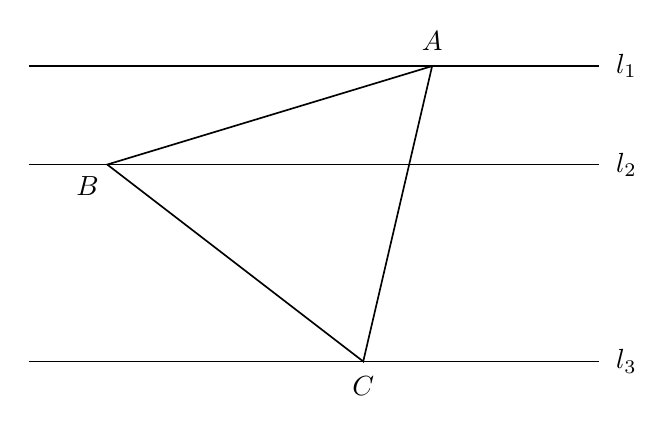
\begin{tikzpicture}[scale=1.25, semithick,
  every node/.style={inner sep=1.5pt}]
  % 三条平行线
  \draw (-0.2,2.2) -- (5.6,2.2);
  \draw (-0.2,1.2) -- (5.6,1.2);
  \draw (-0.2,-0.8) -- (5.6,-0.8);
  % 正三角形的三个顶点
  \coordinate (A) at (3.9,2.2);
  \coordinate (B) at (0.6,1.2);
  \coordinate (C) at (3.2,-0.8);
  \draw (A) -- (B) -- (C) -- cycle;
  \node[anchor=west] at (5.72,2.2) {$l_1$};
  \node[anchor=west] at (5.72,1.2) {$l_2$};
  \node[anchor=west] at (5.72,-0.8) {$l_3$};
  \node[anchor=south] at ([yshift=3pt]A) {$A$};
  \node[anchor=north east] at ([xshift=-1pt,yshift=-2pt]B) {$B$};
  \node[anchor=north] at ([yshift=-3pt]C) {$C$};
\end{tikzpicture}
